\documentclass[12pt,thmsa]{article}

%maths
\usepackage{amsmath}   % \sideset
\usepackage{amsthm}    % for proof
\usepackage{amsfonts}  % for \mathbb
\usepackage{mathrsfs}  % for Ralph Smith's Formal Script Font
\usepackage[mathscr]{euscript} %redefine the \mathcal command to use Euler script
\usepackage{amssymb}   % \varnothing, \bigstar, \blacksquare, \clubsuit, \blacktriangleright, \diamondsuit, \spadesuit, \dagger, \checkmark

%algorithms
\usepackage{algorithm} % http://ctan.org/pkg/algorithms
\usepackage{algpseudocode}% http://ctan.org/pkg/algorithmicx

%tables
\usepackage{booktabs}  % Allows the use of \toprule, \midrule and \bottomrule in tables
\usepackage{multirow}
\usepackage{multicol}
\usepackage{tabularx}
\usepackage[table]{xcolor} % For \cellcolor
\usepackage[export]{adjustbox}

%figures
\usepackage{graphicx}  % Allows including images
\usepackage{float}     % Force figure placement in text with [H]

%tikzpicture
\usepackage{tikz}
\usepackage{scalerel}
\usepackage{pict2e}
\usepackage{tkz-euclide}
\usetikzlibrary{matrix}
\usetikzlibrary{shapes, positioning}
\usetikzlibrary{calc}
\usetikzlibrary{patterns, arrows.meta}
\usetikzlibrary{shadows}
\usetikzlibrary{external}

%pgfplots
\usepackage{pgfplots}
\pgfplotsset{compat=newest}
\usepgfplotslibrary{statistics}
\usepgfplotslibrary{fillbetween}
% Define layers for drawing the dashed lines behind the plot
\pgfdeclarelayer{bg}   % declare background layer
\pgfsetlayers{bg,main}  % set the order of the layers (main is the standard layer)

%colors
\usepackage{color}

%other
\usepackage{cancel}
\usepackage{enumitem}
\setlist[itemize]{leftmargin=*} % global option, remove the indentation for a specific list
\usepackage{textcase}  % \MakeTextUppercase
\renewcommand{\qedsymbol}{$\blacksquare$} % change the QED symbol to a filled square
\usepackage{hyperref}
\usepackage{extarrows} % \xLongrightarrow

%layout
\usepackage{geometry}

\geometry{
	a4paper,
	total={170mm,257mm},
	left=20mm,
	right=20mm,
	top=20mm,
}

% Linhui added for newly defined color
\definecolor{forestgreen}{RGB}{34,139,34}

% Linhui added for Expectation and Variance
\newcommand{\Exp}{{\mathbb E}\! }
\newcommand{\Var}{\mbox{Var}\! }

% Linhui added for rename the command for empty set.
\let\oldemptyset\emptyset
\let\emptyset\varnothing


%------------------------------------------------------%
\makeatletter
\def\maketitle{%
	\par
	\hrule height 1.5pt\vspace{1ex}
	\par\noindent
	
	\begin{minipage}{0.5\textwidth}
		\scshape
		Purdue University $\cdot$ ece 58000 \\[1ex]
		Optimization Methods \\
		Prof. Żak, Prof. Chong
	\end{minipage}
	\begin{minipage}{0.45\textwidth}
		\raggedleft
		\MakeTextUppercase{{\@title}}\\[0.3ex] % 0.2ex height space between two line
		\textit{\@author}\\[0.2ex]
		\textit{December 1, 2022}
	\end{minipage}
	\par\vspace{1ex}
	\hrule height 1.5pt\vspace{1ex}
	\par
}
\makeatother

\author{Linhui Xie}
\title{Lecture Note 06}
%------------------------------------------------------%

\begin{document}
\maketitle
\setcounter{section}{5}
%------------------------------------------------------%
\section{Basics for optimization\medskip}
%------------------------------------------------------%
\setcounter{section}{6}


%------------------------------------------------------%
\subsection{Introduction}
%------------------------------------------------------%
\begin{itemize}
	\item Optimization problem:
	\[
		\begin{array}{rl}
			\operatorname{minimize} & f(\boldsymbol{x}) \\
			\text { subject to} & \boldsymbol{x} \in \Omega
		\end{array}
	\]
	\begin{itemize}
	\item[\(\circ\)] \(\Omega\) : \underline{constraint} set or \underline{feasible set}.
	
	\item[\(\circ\)]  \(f(\boldsymbol{x})\) is called the \underline{objective function} or \underline{cost function};

	\item[\(\circ\)]  \(\Omega=\mathbb{R}^n\): \textbf{unconstrained} minimization.
	
	\item[\(\circ\)]  \(\Omega \subset \mathbb{R}^n\) explicitly given: set \textbf{constrained} minimization.
	
	\item[\(\circ\)] \(\Omega=\left\{\boldsymbol{x} \in \mathbb{R}^n: g(\boldsymbol{x})=0, h(\boldsymbol{x}) \leq 0\right\}:\) functional \textbf{constrained} minimization.

	\item[\(\circ\)] Solution to the problem: a minimizer, \(\boldsymbol{x}^{*}\).
	
	\end{itemize}

	
	\item \underline{Global minimizer}: \(f\left(\boldsymbol{x}^{*}\right) \leq f(\boldsymbol{x})\) for all \(\boldsymbol{x} \in \Omega \backslash\left\{\boldsymbol{x}^{*}\right\}\).
	
	\item \underline{Local minimizer}: there exists \(\varepsilon>0\) such that \(f\left(\boldsymbol{x}^{*}\right) \leq f(\boldsymbol{x})\) for all \(\boldsymbol{x} \in \Omega \) and \(\left\|\boldsymbol{x}-\boldsymbol{x}^{*}\right\|<\varepsilon\).
	
	\item \underline{\textbf{Strict} global minimizer}: \(f\left(\boldsymbol{x}^{*}\right) {\color{forestgreen}<} f(\boldsymbol{x})\) for all \(\boldsymbol{x} \in \Omega \backslash\left\{\boldsymbol{x}^{*}\right\}\).

	\item \underline{\textbf{Strict} local minimizer}: there exists \(\varepsilon>0\) such that \(f\left(\boldsymbol{x}^{*}\right) {\color{forestgreen}<} f(\boldsymbol{x})\) for all \(\boldsymbol{x} \in \Omega \backslash\left\{\boldsymbol{x}^{*}\right\}\) and \(\left\|\boldsymbol{x}-\boldsymbol{x}^{*}\right\|<\varepsilon\).
	
\end{itemize}


\begin{itemize}
	\item \(\mathscr{THEOREM}\) 4.2 Theorem of Weierstrass: If \(f\) is continuous and \(\Omega\) is \textit{closed} and \textit{bounded}, then a global minimizer exists.
\end{itemize}

%------------------------------------------------------%
\subsection{Conditions: Necessary and Sufficient}
\begin{itemize}
	
	\item Two types of conditions: \underline{necessary} and \underline{sufficient}, that characterize minimizers.
	
	\item \textit{Necessary} condition \(\Longleftarrow\): If \(\boldsymbol{x}^{*}\) is a minimizer, then \(\boldsymbol{x}^{*}\) satisfies this particular condition.
	
	\item \textit{Sufficient} condition \(\Longrightarrow\): If \(\boldsymbol{x}^{*}\) satisfies this particular condition, then \(\boldsymbol{x}^{*}\) is a minimizer.
	
	\item A \textit{necessary} condition limits the set of candidates for minimizers.
	
	\item A \textit{sufficient} condition guarantees that a point is a minimizer.
	
	\item In this course, consider conditions that are based on \textbf{gradients} and \textbf{Hessians} and apply these conditions to local minimizers.
	
\end{itemize}


%------------------------------------------------------%
\subsection{Reminder methods of proof}

\begin{enumerate}
	\item By direct method, \[ S_{1} \Longrightarrow S_{2}.  \]
	\item By contraposition, \[ \begin{array}{rcl} S_{1} & \Longrightarrow & S_{2}, \\ & \Updownarrow &\\ \left( \text{ NOT } S_{2}\right) & \Longrightarrow & \left(\text { NOT } S_{1}\right). \end{array}\]
	\item By contradiction, \[ \begin{array}{rcl} S_{1} & \Longrightarrow & S_{2}, \\ & \Updownarrow & \\ \text{NOT } \Big(S_1, &\text{ AND }& (\text{ NOT } S_2 ) \Big). \end{array} \]

\end{enumerate}



%------------------------------------------------------%
\subsection{Conditions for local minimizers}
\begin{itemize}
	\item An \textbf{unconstrained} problem, with assumption \(f \in \mathcal{C}^{1}\), a real valued function on \( \mathbb{R}^{n}\):
	\[
	\begin{aligned}
		\text { minimize }   & f(\boldsymbol{x}) \\
		\text { subject to } & \boldsymbol{x} \in \mathbb{R}^{n} .
	\end{aligned}
	\]
	
	\item[\(\spadesuit\)] \(\mathscr{THEOREM}\) If \(\boldsymbol{x}^{*}\) is a local minimizer, then
	\[
	\nabla f\left(\boldsymbol{x}^{*}\right)=\mathbf{0} .
	\]
	
	\item An \textbf{constrained} problem, with assumption \(f \in \mathcal{C}^{1}\), a real valued function on \( \Omega \):
	\[
	\begin{aligned}
		\text { minimize }   & f(\boldsymbol{x}) \\
		\text { subject to } & \boldsymbol{x} \in \Omega .
	\end{aligned}
	\]

	\item[\(\spadesuit\)] \(\mathscr{COROLLARY}\) 6.1 If \(\boldsymbol{x}^{*}\) is a local minimizer and an interior point of \(\Omega\), then
	\[
	\nabla f\left(\boldsymbol{x}^{*}\right)=\mathbf{0} .
	\]
	\[ \fbox{\vspace{1em}\hspace{1em}
		\(\begin{array}{ccccc}
			\text{ interior point } \boldsymbol{x}^* \text{ is a local minimizer, } & & \xLongrightarrow{\text{ FONC }} & & \nabla f\left(\boldsymbol{x}^{*}\right)=\mathbf{0}.
		\end{array}
		\)
	}
	\]
	
\end{itemize}


\begin{itemize}
	\item Proof of theorem (by contraposition): suppose \(\nabla f\left(\boldsymbol{x}^{*}\right) \neq \mathbf{0}\).
	
	\begin{itemize}
		\item[\(\circ\)] Since \( {\color{forestgreen}-} \nabla f\left(\boldsymbol{x}^{*}\right)\) points in the direction of {\color{forestgreen}decreasing} \(f\), there will be some points close to \(\boldsymbol{x}^{*}\) that have smaller \(f\) value.
		
		\item[\(\circ\)] Specifically, consider \(\boldsymbol{x}_{\alpha}=\boldsymbol{x}^{*}-\alpha \nabla f\left(\boldsymbol{x}^{*}\right), \alpha>0\).
		
		\item[\(\circ\)] From an equation derived by Taylor's formula,
		\[
		f\left(\boldsymbol{x}_{\alpha}\right)=f\left(\boldsymbol{x}^{*}\right)-\alpha\left\|\nabla f\left(\boldsymbol{x}^{*}\right)\right\|^{2}+o(\alpha) .
		\]
		\[f\left(\boldsymbol{x}_{\alpha}\right)<f\left(\boldsymbol{x}^{*}\right).\]
		\[ \begin{array}{ccccc}
			\neg S_{2} & & & & \neg S_{1} \\
			\nabla f\left(\boldsymbol{x}^{*}\right) \neq \mathbf{0}, & & {\color{forestgreen}\xLongrightarrow{}}  & & \boldsymbol{x}^* \text{  is definitely not a local minimizer. } \\
			& &  \Updownarrow & & \\
			S_{1} & & & & S_{2} \\
			\boldsymbol{x}^* \text{  is a local minimizer, }  & & {\color{forestgreen}\xLongrightarrow{}}  & & \nabla f\left(\boldsymbol{x}^{*}\right) = \mathbf{0} . \\
		\end{array}
		\]
	\end{itemize}
	
\end{itemize}


%------------------------------------------------------%
\subsection{Feasible directions}
\begin{itemize}
	\item We only consider a nonzero vector \(\boldsymbol{d} \in \mathbb{R}^{n}\).
	
	\item \(\boldsymbol{d}\) is a \underline{feasible direction} at \(\boldsymbol{x} \in \Omega\) if there exists \(\alpha_{0}>0\) such that \(\boldsymbol{x}+\alpha \boldsymbol{d} \in \Omega\) for all \(\alpha \in\left[0, \alpha_{0}\right]\).
	
	\item At an \textit{interior} point, all directions are feasible.
	
	\item At a \textit{boundary} point, only some directions ``point interior points of " the set are feasible. 
	
\end{itemize}

\begin{center}
	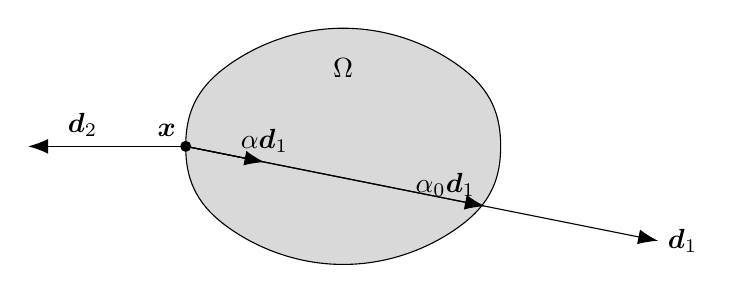
\begin{tikzpicture}[>={Latex[scale=1.5]}] % Scale the arrow tip
		% Draw the shape for space
		\draw[fill=gray!30] plot[smooth cycle, tension=0.7] coordinates {
			(-2, 0) (-1.5, 1) (0, 1.5) (1.5, 1) (2, 0) (1.5, -1) (0, -1.5) (-1.5, -1)
		};
		
		% space omega
		\node at (0, 1) {\(\Omega\)};
		%\node at (-2.2, 0.2) {\(x\)};
		
		% point x
		\fill (-2,0) circle (2pt) node[above left] {\(\boldsymbol{x}\)};
		
		% Draw the d1 arrow
		\draw[->] (-2, 0) -- node[at end, right] {\(\boldsymbol{d}_1\)} (4, -1.2);
		
		% Draw the alpha d1 arrow
		\draw[->] (-2, 0) -- node[at end, above] {\(\alpha \boldsymbol{d}_1\)} (-1, -0.2);
		
		% Draw the alpha_0 d1 arrow
		\draw[->] (-2, 0) -- node[at end, above left] {\(\alpha_0 \boldsymbol{d}_1\)} (1.8, -0.76);
		
		% Draw the d2 arrow
		\draw[->] (-2, 0) -- node[above left] {\(\boldsymbol{d}_2\)} (-4, 0);
		
	\end{tikzpicture}
\end{center}

\begin{itemize}
	\item \(\boldsymbol{d}_1\) is a feasible direction, whereas \(\boldsymbol{d}_2\) is not a feasible direction.
\end{itemize}


%------------------------------------------------------%
\subsection{First order necessary conditions}

\begin{itemize}
	\item \(\mathscr{THEOREM}\) 6.1 (FONC) If \(\boldsymbol{x}^{*}\) is a local minimizer, then
	
	\[
		\boldsymbol{d}^{\top} \nabla f\left(\boldsymbol{x}^{*}\right) \geq \mathbf{0}
	\]
	
	for all feasible directions \(\boldsymbol{d}\).
	
	\[ \fbox{\vspace{1em}\hspace{1em}
		\(\begin{array}{ccccc}
			\boldsymbol{x}^* \text{ is a local minimizer, } & & \xLongrightarrow{\text{ FONC }} & & \boldsymbol{d}^{\top} \nabla f(\boldsymbol{x}^*) \geq 0, \text{ for all feasible } \boldsymbol{d}.
		\end{array}
		\)
	}
	\]
\end{itemize}


\begin{center}
	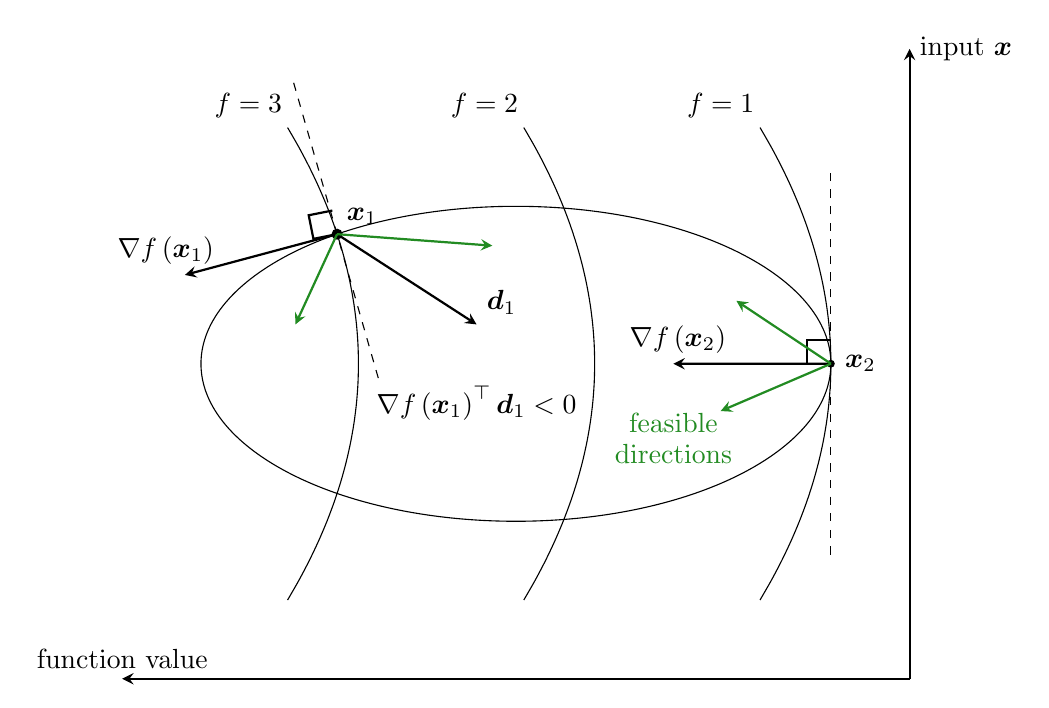
\begin{tikzpicture}[scale=1,>=stealth]
		
		% draw an ellipse
		\draw[name path=ellipse] (0,0) ellipse (4cm and 2cm);	
		% If need the ellipse rotated by 10 degrees
		% \draw[name path=ellipse, rotate around={10:(0,0)}] (0,0) ellipse (4cm and 2cm);
		
		% Name the path without drawing it, and then 
		% draw parabolic contour curve that mimics y^2 + c = x
		\path[name path=f1] plot[domain=-3:3, smooth, variable=\y] ({-\y*\y/10 + 4}, {\y});
		\draw[domain=-3:3, smooth, variable=\y,  black] plot ({-\y*\y/10 + 4}, {\y})
			node[right, above, xshift=-0.5cm] {\(f=1\)};
			
		\path[name path=f2] plot[domain=-3:3, smooth, variable=\y] ({-\y*\y/10 + 1}, {\y});
		\draw[domain=-3:3, smooth, variable=\y,  black] plot ({-\y*\y/10 + 1}, {\y})
			node[right, above, xshift=-0.5cm] {\(f=2\)};
		
		\path[name path=f3] plot[domain=-3:3, smooth, variable=\y] ({-\y*\y/10 - 2}, {\y});
		\draw[domain=-3:3, smooth, variable=\y,  black] plot ({-\y*\y/10 - 2}, {\y})
			node[right, above, xshift=-0.5cm] {\(f=3\)};

		% Find the position of x2 on the ellipse
		\draw[name intersections={of=ellipse and f1, by=x2}] 
		(x2) node[circle, fill, inner sep=1pt, label={right:\(\boldsymbol{x}_2\)}] {};
		
		% Find the intersection points of the ellipse and the contour line
		\path [name intersections={of=ellipse and f3, by={x1,int2}}];
		
		% Mark the intersection points
		\fill[black] (x1) circle (2pt) node[above right] {\(\boldsymbol{x}_1\)};
		
		% Draw an approximate dashed tangent vector at x1
		\draw[dashed] ($(x1)!-2cm!(-1.8,0)$) -- ($(x1)!2cm!(-1.8,0)$);
		
		% Draw the dashed lines extending from x2
		\draw[dashed] (x2) -- +(0,2.5);
		\draw[dashed] (x2) -- +(0,-2.5);
		
		% Draw the approximate gradient arrow
		% \draw[->, thick] (x1) -- node[at end, above left, xshift=0.5cm] {\(\nabla f\left(\boldsymbol{x}_1\right)\)} (-4, 1.4);
		\draw[thick, ->] (x1) -- ++(195:2cm) node[at end, above left, xshift=0.5cm] {\(\nabla f\left(\boldsymbol{x}_1\right)\)};
		\draw[->, thick] (x2) -- node[at end, above left, xshift=0.8cm] {\(\nabla f\left(\boldsymbol{x}_2\right)\)} (2, 0);
		
		% Mark the intersection point x2 with an L-shape
		\draw[thick] (x2) -- ++(-0.3,0) -- ++(0,0.3) -- ++(0.3,0);
		\draw[thick] (x1) -- ++(-0.3,-0.06) -- ++(-0.06,0.3) -- ++(0.3,0.06);
		
		% Draw the d arrow
		\draw[->, thick] (x1) -- node[at end, above right] {\(\boldsymbol{d}_1\)} (-0.5, 0.5);
		\node at (-0.5, -0.5) {\(\nabla f\left(\boldsymbol{x}_1\right)^{\top} \boldsymbol{d}_1 < 0\)};
		
		% Draw the feasible directions
		\draw[->, thick, forestgreen] (x1) -- node[at end, above right] {} (-0.3, 1.5);
		\draw[->, thick, forestgreen] (x1) -- node[at end, above right] {} (-2.8, 0.5);
		\draw[->, thick, forestgreen] (x2) -- node[at end, above right] {} (2.8, 0.8);
		\draw[->, thick, forestgreen] (x2) -- node[at end, above right] {} (2.6, -0.6);
		\fill[forestgreen] (2,-0.5) node[below] {feasible};
		\fill[forestgreen] (2,-0.9) node[below] {directions};
		
		% Draw the vertical-axis and horizontal-axis arrow
		\draw[->, thick] (5, -4) -- node[at end, right] {\(\text{input } \boldsymbol{x}\)} (5, 4);
		\draw[->, thick] (5, -4) -- node[at end, above] {\(\text{function value}\)} (-5, -4);
	\end{tikzpicture}
\end{center}


\begin{itemize}
	
	\item \(\boldsymbol{x}_1\) does not satisfy FONC, but \(\boldsymbol{x}_2\) satisfies FONC.
	
	\item If \(\boldsymbol{x}^{*}\) is a local minimizer, then the \textit{directional derivative} of \(f\) in any feasible direction must be \(\geq 0\) (since the function must be increasing in that direction).
	
%	\item In the interior case, the general FONC reduces to \(\nabla f\left(\boldsymbol{x}^{*}\right)=\mathbf{0}\).
	
	\item General case: \(\boldsymbol{d}^{\top} \nabla f\left(\boldsymbol{x}^{*}\right) \geq \mathbf{0}\) for all feasible directions \(\boldsymbol{d}\).
	
\end{itemize}


\begin{itemize}
	
	\item Example: consider the constrained problem
	\[
	\begin{array}{rl}
		\operatorname{minimize} & f(\boldsymbol{x}) \\
		\text { subject to } & \boldsymbol{x} \in \Omega
	\end{array}
	\]where \(f \in \mathcal{C}^{2} \), \(f: \mathbb{R}^{2} \rightarrow \mathbb{R}, \Omega=\left\{\boldsymbol{x}=\left[x_{1}, x_{2}\right]^{\top}: x_{1} \geq 1\right\}, \boldsymbol{x}^{*}=[1,2]^{\top} \), and gradient \(\nabla f\left(\boldsymbol{x}^{*}\right)=[1,1]^{\top} \). Determine the type of minimizer for the given point \(\boldsymbol{x}^{*}\).
	
	\textbf{Short answer},
	
	\begin{itemize}
		\item[\(\circ\)] For \(\boldsymbol{x}^* = \begin{bmatrix} 1 \\ 2 \end{bmatrix}\), exists a \textit{feasible direction} \(\boldsymbol{d} = \begin{bmatrix} 1 \\ -5 \end{bmatrix}\),
	
		\[
		\exists \ \alpha_{0} = 1 > 0, \text{ s.t. } \boldsymbol{x}^* + \alpha \boldsymbol{d} = \begin{bmatrix} 1+\alpha \\ 2-5\alpha \end{bmatrix} \in \Omega, \text{ for all } \alpha \in\left[0, \alpha_{0}\right]. 
		\]
	
		\item[\(\circ\)] However,
		\[
		\boldsymbol{d}^{\top} \nabla f(\boldsymbol{x}^*) = \begin{bmatrix} 1 & -5 \end{bmatrix} \begin{bmatrix} 1 \\ 1 \end{bmatrix} = -4 < 0
		\]
		violates the FONC.
		\[ \begin{array}{ccccc}
			S_{1} & & & & S_{2} \\
			\boldsymbol{x}^* \text{ is a local minimizer, } & & { \color{forestgreen}\xLongrightarrow{{\color{black}\text{ FONC }}} } & & \boldsymbol{d}^{\top} \nabla f(\boldsymbol{x}^*) \geq 0, \text{ for all feasible } \boldsymbol{d}.
			\end{array}
		\]
		\item[\(\circ\)] Based on truth table and by contraposition,
		\[ S_{1} {\color{forestgreen}\Rightarrow}  S_{2}, \quad \mathbf{\xLongleftrightarrow{}} \quad \neg S_{2} {\color{forestgreen}\Rightarrow} \neg S_{1}. \]
		\[ \begin{array}{ccccc}
			 	\neg S_{2} & & & & \neg S_{1} \\
			 \boldsymbol{d}^{\top} \nabla f(\boldsymbol{x}^*) < 0, \text{ for some } \boldsymbol{d}, & & {\color{forestgreen}\xLongrightarrow{}}  & & \boldsymbol{x}^* \text{  is definitely not a local minimizer. }
			\end{array}
		\]
	\end{itemize}
\end{itemize}



\bigskip

\noindent
[Ref]: Edwin K.P. Chong, Stanislaw H. Żak, ``PART II UNCONSTRAINED OPTIMIZATION" in ``\href{https://www.amazon.com/Introduction-Optimization-Edwin-K-Chong/dp/1118279018}{An introduction to optimization}", 4th Edition, John Wiley and Sons, Inc. 2013.


\end{document}
